\documentclass[11pt]{article}

\usepackage[margin=1in]{geometry}
\usepackage[T1]{fontenc}
\usepackage{graphicx}
\usepackage{longtable}
\usepackage{booktabs}
\usepackage{array}
\usepackage{enumitem}
\usepackage{xcolor}
\usepackage{hyperref}
\usepackage{tikz}
\usepackage{float}
\usepackage{fancyhdr}
\usepackage{titlesec}
\usepackage{tcolorbox}
\usepackage{tabularx}
\usepackage{multirow}
\usepackage{caption}
\usepackage{makecell}
\usepackage{amssymb}
\usepackage{pifont}

\usetikzlibrary{shapes.geometric, arrows.meta, positioning, fit, backgrounds, calc, decorations.pathreplacing, shapes.multipart, matrix, shadows}

% ---------------------------------------------------------------------------
% Color Definitions
% ---------------------------------------------------------------------------
\definecolor{sectionblue}{RGB}{31,78,121}
\definecolor{dodafcolor}{RGB}{0,102,153}
\definecolor{vbcolor}{RGB}{60,179,113}
\definecolor{allviewcolor}{RGB}{128,128,128}
\definecolor{opviewcolor}{RGB}{255,165,0}
\definecolor{svviewcolor}{RGB}{70,130,180}
\definecolor{tvviewcolor}{RGB}{186,85,211}
\definecolor{flowcolor}{RGB}{100,100,100}
\definecolor{lightgray}{RGB}{245,245,245}
\definecolor{warningred}{RGB}{220,53,69}
\definecolor{successgreen}{RGB}{40,167,69}
\definecolor{infoblue}{RGB}{23,162,184}
\definecolor{modulecolor}{RGB}{144,238,144}
\definecolor{cnccolor}{RGB}{255,182,193}
\definecolor{alloccolor}{RGB}{173,216,230}

\hypersetup{
  colorlinks=true,
  linkcolor=sectionblue,
  urlcolor=sectionblue,
  citecolor=sectionblue
}

% ---------------------------------------------------------------------------
% Header and Footer
% ---------------------------------------------------------------------------
\pagestyle{fancy}
\fancyhf{}
\fancyhead[L]{\leftmark}
\fancyhead[R]{DoDAF and Views \& Beyond Integration Guide}
\fancyfoot[C]{\thepage}
\renewcommand{\headrulewidth}{0.4pt}
\renewcommand{\footrulewidth}{0.4pt}

% ---------------------------------------------------------------------------
% Section Formatting
% ---------------------------------------------------------------------------
\titleformat{\section}
  {\normalfont\Large\bfseries\color{sectionblue}}{\thesection}{1em}{}
\titleformat{\subsection}
  {\normalfont\large\bfseries\color{sectionblue!80}}{\thesubsection}{1em}{}
\titleformat{\subsubsection}
  {\normalfont\normalsize\bfseries\color{sectionblue!60}}{\thesubsubsection}{1em}{}

% ---------------------------------------------------------------------------
% Custom Box Environments
% ---------------------------------------------------------------------------
\newtcolorbox{keypoint}{
    colback=blue!5,
    colframe=sectionblue,
    title=Key Point,
    fonttitle=\bfseries
}

\newtcolorbox{warning}{
    colback=red!5,
    colframe=warningred,
    title=Warning,
    fonttitle=\bfseries
}

\newtcolorbox{bestpractice}{
    colback=green!5,
    colframe=successgreen,
    title=Best Practice,
    fonttitle=\bfseries
}

\newtcolorbox{example}{
    colback=lightgray,
    colframe=flowcolor,
    title=Example,
    fonttitle=\bfseries
}

\newtcolorbox{definition}{
    colback=infoblue!10,
    colframe=infoblue,
    title=Definition,
    fonttitle=\bfseries
}

\newtcolorbox{dodafbox}[1][]{
    colback=dodafcolor!8,
    colframe=dodafcolor,
    title=#1,
    fonttitle=\bfseries,
    breakable
}

\newtcolorbox{vbbox}[1][]{
    colback=vbcolor!10,
    colframe=vbcolor,
    title=#1,
    fonttitle=\bfseries,
    breakable
}

\newtcolorbox{mappingbox}[1][]{
    colback=opviewcolor!10,
    colframe=opviewcolor,
    title=#1,
    fonttitle=\bfseries
}

\newtcolorbox{checklistbox}[1][]{
    colback=white,
    colframe=flowcolor,
    title=#1,
    fonttitle=\bfseries
}

\tcbuselibrary{listings}

% ---------------------------------------------------------------------------
% List Settings
% ---------------------------------------------------------------------------
\setlist[itemize]{leftmargin=*,topsep=3pt,itemsep=2pt,parsep=0pt}
\setlist[enumerate]{leftmargin=*,topsep=3pt,itemsep=2pt,parsep=0pt}

% ---------------------------------------------------------------------------
% Custom Column Types
% ---------------------------------------------------------------------------
\newcolumntype{L}[1]{>{\raggedright\arraybackslash}p{#1}}
\newcolumntype{C}[1]{>{\centering\arraybackslash}p{#1}}
\newcolumntype{R}[1]{>{\raggedleft\arraybackslash}p{#1}}

% ---------------------------------------------------------------------------
% Custom Commands
% ---------------------------------------------------------------------------
\newcommand{\dodaf}{\textsc{DoDAF}}
\newcommand{\vb}{Views \& Beyond}
\newcommand{\allview}{\textcolor{allviewcolor}{\textbf{AV}}}
\newcommand{\opview}{\textcolor{opviewcolor}{\textbf{OV}}}
\newcommand{\svview}{\textcolor{svviewcolor}{\textbf{SV}}}
\newcommand{\tvview}{\textcolor{tvviewcolor}{\textbf{TV}}}

% ---------------------------------------------------------------------------
% Title
% ---------------------------------------------------------------------------
\title{%
    \vspace{-1cm}
    \textbf{\Huge Software Architecture Documentation}\\[12pt]
    \Large Integrating DoDAF with Views and Beyond\\[8pt]
    \large A Comprehensive Guide to Mapping DoDAF Products\\
    to Views and Beyond Documentation Practices
}
\author{%
    \textit{Architecture Documentation Series}\\[4pt]
    \small Based on DoDAF 2.02 and SEI Views and Beyond
}
\date{\today}

\begin{document}
\maketitle
\thispagestyle{empty}

\vspace{0.5cm}

\begin{abstract}
\noindent
The Department of Defense Architecture Framework (DoDAF) and the Software Engineering Institute's Views and Beyond approach represent two influential methodologies for architecture documentation. DoDAF provides a standardized framework for defense enterprise architectures, while Views and Beyond offers practical guidance for software architecture documentation. This comprehensive guide provides detailed mappings between DoDAF products and Views and Beyond constructs, enabling architects to leverage the strengths of both approaches. The document covers all DoDAF viewpoints (All View, Operational, Systems and Services, Technical Standards), provides implementation guidance, and includes practical examples demonstrating how to create documentation that satisfies both frameworks simultaneously.
\end{abstract}

\vfill

\begin{center}
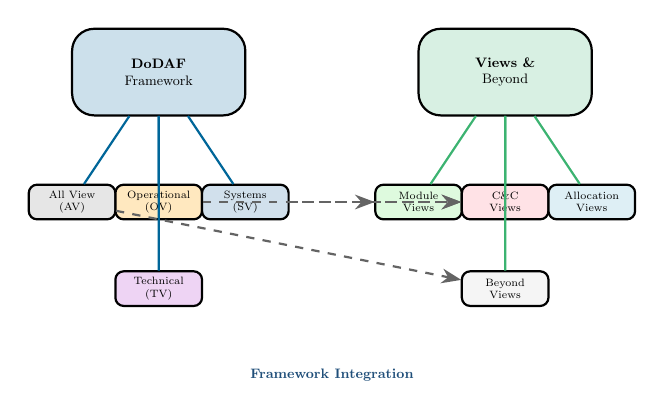
\begin{tikzpicture}[
    scale=0.55,
    transform shape,
    framework/.style={draw, thick, rounded corners=8pt, minimum width=4cm, minimum height=2cm, font=\small, align=center},
    product/.style={draw, thick, rounded corners=3pt, minimum width=2cm, minimum height=0.8cm, font=\scriptsize, align=center},
    arrow/.style={-{Stealth[length=2.5mm]}, thick}
]
    % DoDAF side
    \node[framework, fill=dodafcolor!20] (dodaf) at (-4,3) {\textbf{DoDAF}\\Framework};
    \node[product, fill=allviewcolor!20] (av) at (-6,0) {All View\\(AV)};
    \node[product, fill=opviewcolor!25] (ov) at (-4,0) {Operational\\(OV)};
    \node[product, fill=svviewcolor!25] (sv) at (-2,0) {Systems\\(SV)};
    \node[product, fill=tvviewcolor!25] (tv) at (-4,-2) {Technical\\(TV)};
    
    % Views and Beyond side
    \node[framework, fill=vbcolor!20] (vb) at (4,3) {\textbf{Views \&}\\Beyond};
    \node[product, fill=modulecolor!30] (mod) at (2,0) {Module\\Views};
    \node[product, fill=cnccolor!40] (cnc) at (4,0) {C\&C\\Views};
    \node[product, fill=alloccolor!40] (alloc) at (6,0) {Allocation\\Views};
    \node[product, fill=lightgray] (beyond) at (4,-2) {Beyond\\Views};
    
    % Connections from frameworks
    \draw[thick, dodafcolor] (dodaf) -- (av);
    \draw[thick, dodafcolor] (dodaf) -- (ov);
    \draw[thick, dodafcolor] (dodaf) -- (sv);
    \draw[thick, dodafcolor] (dodaf) -- (tv);
    
    \draw[thick, vbcolor] (vb) -- (mod);
    \draw[thick, vbcolor] (vb) -- (cnc);
    \draw[thick, vbcolor] (vb) -- (alloc);
    \draw[thick, vbcolor] (vb) -- (beyond);
    
    % Mapping arrows
    \draw[arrow, dashed, flowcolor] (ov) -- (cnc);
    \draw[arrow, dashed, flowcolor] (sv) -- (cnc);
    \draw[arrow, dashed, flowcolor] (sv) -- (mod);
    \draw[arrow, dashed, flowcolor] (av) -- (beyond);
    
    % Label
    \node[font=\bfseries\small, text=sectionblue] at (0,-4) {Framework Integration};
\end{tikzpicture}
\end{center}

\newpage
\tableofcontents
\newpage

%==============================================================================
\section{Introduction}
%==============================================================================

\subsection{Purpose of This Guide}

This guide provides comprehensive guidance for integrating the Department of Defense Architecture Framework (DoDAF) with the Views and Beyond approach to software architecture documentation. Organizations using DoDAF can benefit from the practical documentation techniques in Views and Beyond, while organizations using Views and Beyond can ensure their documentation meets DoDAF requirements when needed.

\subsection{About the Frameworks}

\begin{definition}
\textbf{DoDAF (Department of Defense Architecture Framework)} is a standardized approach for developing and presenting enterprise architectures within the U.S. Department of Defense. It defines a set of viewpoints and products that describe architectures from multiple perspectives.
\end{definition}

\begin{definition}
\textbf{Views and Beyond} is an approach to software architecture documentation developed by the Software Engineering Institute (SEI). It emphasizes stakeholder-driven documentation using architectural views selected to address specific concerns.
\end{definition}

\subsection{Why Integrate Both Approaches?}

\begin{keypoint}
\textbf{Complementary Strengths:}

\begin{itemize}
    \item \textbf{DoDAF} provides a comprehensive enterprise architecture framework with standardized products required for defense acquisitions
    \item \textbf{Views and Beyond} provides practical guidance for documenting software architectures with emphasis on stakeholder needs and quality attributes
    \item Together, they enable documentation that satisfies acquisition requirements while being useful for development teams
\end{itemize}
\end{keypoint}

\subsection{Document Organization}

\begin{itemize}
    \item \textbf{Section 2:} Framework overviews
    \item \textbf{Section 3:} All View (AV) mappings
    \item \textbf{Section 4:} Operational View (OV) mappings
    \item \textbf{Section 5:} Systems and Services View (SV) mappings
    \item \textbf{Section 6:} Technical Standards View (TV) mappings
    \item \textbf{Section 7:} Implementation guidance
    \item \textbf{Appendices:} Complete mapping tables, templates, and references
\end{itemize}

%==============================================================================
\section{Framework Overviews}
%==============================================================================

\subsection{DoDAF Overview}

DoDAF organizes architecture descriptions into viewpoints, each containing multiple products (models):

\begin{figure}[H]
\centering
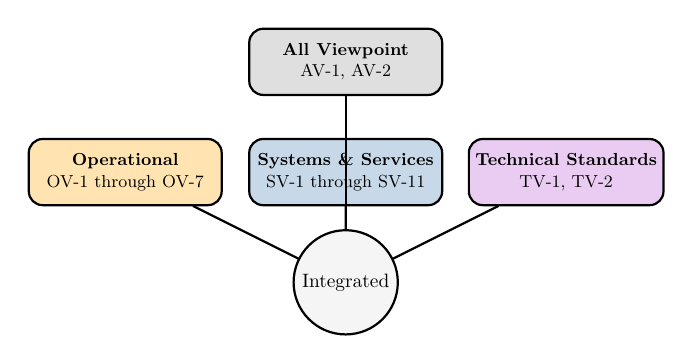
\begin{tikzpicture}[
    scale=0.7,
    transform shape,
    viewpoint/.style={draw, thick, fill=#1, minimum width=3.5cm, minimum height=1.2cm, rounded corners=5pt, font=\small, align=center},
    arrow/.style={-{Stealth[length=2mm]}, thick}
]
    % Viewpoints
    \node[viewpoint=allviewcolor!25] (av) at (0,4) {\textbf{All Viewpoint}\\AV-1, AV-2};
    \node[viewpoint=opviewcolor!30] (ov) at (-4,2) {\textbf{Operational}\\OV-1 through OV-7};
    \node[viewpoint=svviewcolor!30] (sv) at (0,2) {\textbf{Systems \& Services}\\SV-1 through SV-11};
    \node[viewpoint=tvviewcolor!30] (tv) at (4,2) {\textbf{Technical Standards}\\TV-1, TV-2};
    
    % Central integration
    \node[draw, thick, fill=lightgray, circle, minimum size=1.5cm] (int) at (0,0) {Integrated};
    
    % Connections
    \draw[thick] (av) -- (int);
    \draw[thick] (ov) -- (int);
    \draw[thick] (sv) -- (int);
    \draw[thick] (tv) -- (int);
\end{tikzpicture}
\caption{DoDAF Viewpoints}
\end{figure}

\begin{longtable}{@{}L{2.5cm} L{4cm} L{6cm}@{}}
\caption{DoDAF Viewpoints Summary} \\
\toprule
\textbf{Viewpoint} & \textbf{Focus} & \textbf{Key Products} \\
\midrule
\endfirsthead
\bottomrule
\endlastfoot
All Viewpoint (AV) & Overview and dictionary & AV-1 Overview; AV-2 Dictionary \\
Operational (OV) & Mission and business processes & OV-1 Concept; OV-2 Connectivity; OV-3 Information Exchange; OV-4 Organization; OV-5 Activity; OV-6 Rules/State/Trace; OV-7 Data Model \\
Systems \& Services (SV) & Systems and services supporting operations & SV-1 Interface; SV-2 Communications; SV-3 Matrix; SV-4 Functionality; SV-5 Traceability; SV-6 Data Exchange; SV-7 Performance; SV-8 Evolution; SV-9 Technology; SV-10 Behavior; SV-11 Schema \\
Technical Standards (TV) & Standards and forecasts & TV-1 Profile; TV-2 Forecast \\
\end{longtable}

\subsection{Views and Beyond Overview}

Views and Beyond organizes architecture documentation into three view categories plus documentation beyond views:

\begin{figure}[H]
\centering
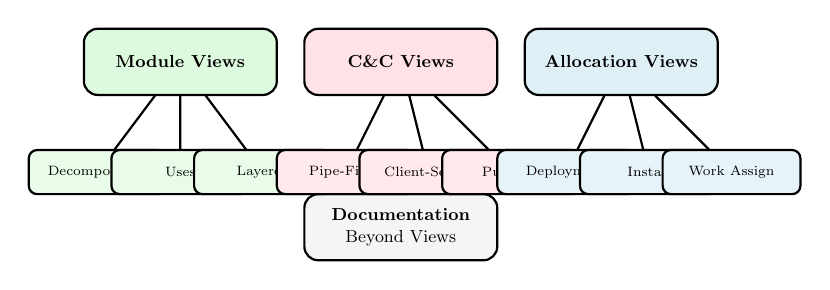
\begin{tikzpicture}[
    scale=0.7,
    transform shape,
    category/.style={draw, thick, fill=#1, minimum width=3.5cm, minimum height=1.2cm, rounded corners=5pt, font=\small, align=center},
    viewtype/.style={draw, thick, fill=#1, minimum width=2.5cm, minimum height=0.8cm, rounded corners=3pt, font=\scriptsize, align=center}
]
    % Categories
    \node[category=modulecolor!30] (mod) at (-4,3) {\textbf{Module Views}};
    \node[category=cnccolor!40] (cnc) at (0,3) {\textbf{C\&C Views}};
    \node[category=alloccolor!40] (alloc) at (4,3) {\textbf{Allocation Views}};
    \node[category=lightgray] (beyond) at (0,0) {\textbf{Documentation}\\Beyond Views};
    
    % View types under Module
    \node[viewtype=modulecolor!20] (decomp) at (-5.5,1) {Decomposition};
    \node[viewtype=modulecolor!20] (uses) at (-4,1) {Uses};
    \node[viewtype=modulecolor!20] (layer) at (-2.5,1) {Layered};
    
    % View types under C&C
    \node[viewtype=cnccolor!30] (pipe) at (-1,1) {Pipe-Filter};
    \node[viewtype=cnccolor!30] (cs) at (0.5,1) {Client-Server};
    \node[viewtype=cnccolor!30] (pub) at (2,1) {Pub-Sub};
    
    % View types under Allocation
    \node[viewtype=alloccolor!30] (deploy) at (3,1) {Deployment};
    \node[viewtype=alloccolor!30] (install) at (4.5,1) {Install};
    \node[viewtype=alloccolor!30] (work) at (6,1) {Work Assign};
    
    % Connections
    \draw[thick] (mod) -- (decomp);
    \draw[thick] (mod) -- (uses);
    \draw[thick] (mod) -- (layer);
    \draw[thick] (cnc) -- (pipe);
    \draw[thick] (cnc) -- (cs);
    \draw[thick] (cnc) -- (pub);
    \draw[thick] (alloc) -- (deploy);
    \draw[thick] (alloc) -- (install);
    \draw[thick] (alloc) -- (work);
\end{tikzpicture}
\caption{Views and Beyond Structure}
\end{figure}

\begin{longtable}{@{}L{2.5cm} L{4cm} L{6cm}@{}}
\caption{Views and Beyond Categories} \\
\toprule
\textbf{Category} & \textbf{Focus} & \textbf{View Types} \\
\midrule
\endfirsthead
\bottomrule
\endlastfoot
Module Views & Code structure and organization & Decomposition, Uses, Generalization, Layered, Data Model, Aspects \\
C\&C Views & Runtime behavior and interaction & Pipe-and-Filter, Client-Server, Peer-to-Peer, Service-Oriented, Publish-Subscribe, Shared-Data \\
Allocation Views & Mapping to environments & Deployment, Install, Work Assignment \\
Beyond Views & Cross-cutting documentation & System Overview, Mapping Between Views, Rationale, Directory \\
\end{longtable}

\subsection{Conceptual Alignment}

\begin{longtable}{@{}L{4cm} L{4cm} L{4.5cm}@{}}
\caption{Conceptual Alignment Between Frameworks} \\
\toprule
\textbf{DoDAF Concept} & \textbf{V\&B Equivalent} & \textbf{Notes} \\
\midrule
\endfirsthead
\bottomrule
\endlastfoot
Viewpoint & Viewtype & Both define conventions for views \\
View/Product & View & Work product expressing architecture \\
Model & Model within View & Specific representation \\
Fit-for-Purpose View & View Packet & Tailored for specific stakeholder \\
Architecture Data & Element Catalog & Detailed element specifications \\
Integrated Dictionary & Glossary & Term definitions \\
\end{longtable}

%==============================================================================
\section{All View (AV) Mappings}
%==============================================================================

The All Viewpoint provides overarching information about the architecture.

\subsection{AV-1: Overview and Summary Information}

\begin{dodafbox}[AV-1: Overview and Summary Information]
\textbf{DoDAF Definition:} Provides executive-level summary information about the architecture including scope, purpose, intended users, environment depicted, and analytical findings.

\textbf{Required Content:}
\begin{itemize}[nosep]
    \item Architecture identification and scope
    \item Purpose and intended use
    \item Context and environment
    \item Analytical findings and recommendations
    \item Architecture status and development approach
\end{itemize}
\end{dodafbox}

\begin{vbbox}[Views and Beyond Equivalent]
\textbf{Primary Mapping:} Documentation Beyond Views

\begin{itemize}
    \item \textbf{Documentation Roadmap:} Explains structure and navigation
    \item \textbf{System Overview:} Provides high-level context
    \item \textbf{Rationale:} Captures analytical findings supporting decisions
    \item \textbf{View Template Introduction:} Purpose and scope of each view
\end{itemize}
\end{vbbox}

\begin{mappingbox}[Implementation Guidance for AV-1]
To satisfy AV-1 using Views and Beyond:

\begin{enumerate}
    \item Create a \textbf{Documentation Roadmap} that:
    \begin{itemize}[nosep]
        \item States architecture identification (name, version, date)
        \item Defines scope boundaries
        \item Lists intended stakeholders
        \item Provides navigation guide to views
    \end{itemize}
    
    \item Create a \textbf{System Overview} that:
    \begin{itemize}[nosep]
        \item Describes system purpose and context
        \item Summarizes key capabilities
        \item Identifies external interfaces
        \item Provides high-level operational concept
    \end{itemize}
    
    \item Include \textbf{Analytical Findings} in:
    \begin{itemize}[nosep]
        \item Rationale sections of views
        \item Architecture Decision Records (ADRs)
        \item Trade study results
    \end{itemize}
\end{enumerate}
\end{mappingbox}

\subsection{AV-2: Integrated Dictionary}

\begin{dodafbox}[AV-2: Integrated Dictionary]
\textbf{DoDAF Definition:} Architecture data repository with definitions of all terms used in all products. Provides a single authoritative source for architecture data elements.

\textbf{Required Content:}
\begin{itemize}[nosep]
    \item Term definitions
    \item Acronym expansions
    \item Data element descriptions
    \item Cross-references between products
\end{itemize}
\end{dodafbox}

\begin{vbbox}[Views and Beyond Equivalent]
\textbf{Primary Mapping:} Glossary and Directory

\begin{itemize}
    \item \textbf{Glossary:} Definitions of all terms
    \item \textbf{Acronym List:} Expansion of abbreviations
    \item \textbf{Element Catalogs:} Detailed element definitions within views
    \item \textbf{Index:} Cross-references to content locations
\end{itemize}
\end{vbbox}

%==============================================================================
\section{Operational View (OV) Mappings}
%==============================================================================

The Operational Viewpoint describes the operational context, activities, and information flows.

\subsection{OV-1: High-Level Operational Concept Graphic}

\begin{dodafbox}[OV-1: High-Level Operational Concept Graphic]
\textbf{DoDAF Definition:} High-level graphical and textual description of the operational concept. Shows key operational nodes, their activities, and interactions.

\textbf{Required Content:}
\begin{itemize}[nosep]
    \item Operational nodes and their missions
    \item Key interactions and information flows
    \item Geographic distribution (if relevant)
    \item Mission context
\end{itemize}
\end{dodafbox}

\begin{vbbox}[Views and Beyond Equivalent]
\textbf{Primary Mapping:} System Overview (Documentation Beyond Views)

The OV-1 maps primarily to the System Overview in the ``documentation beyond views'' section. This provides:
\begin{itemize}
    \item High-level system context
    \item Key operational concepts
    \item Stakeholder relationships
    \item Mission/business purpose
\end{itemize}
\end{vbbox}

\subsection{OV-2: Operational Resource Flow Description}

\begin{dodafbox}[OV-2: Operational Resource Flow Description]
\textbf{DoDAF Definition:} Describes operational nodes, connectivity, and information exchange need lines between nodes.

\textbf{Required Content:}
\begin{itemize}[nosep]
    \item Operational nodes and their roles
    \item Connectivity between nodes
    \item Information exchange requirements
    \item Resource flows
\end{itemize}
\end{dodafbox}

\begin{vbbox}[Views and Beyond Equivalent]
\textbf{Primary Mapping:} Context Diagram

For each operational node scope, create a Context Diagram showing:
\begin{itemize}
    \item System boundary
    \item External entities (other operational nodes)
    \item Information/resource flows between system and externals
    \item This becomes part of a view packet scoped to the node
\end{itemize}
\end{vbbox}

\subsection{OV-3: Operational Resource Flow Matrix}

\begin{dodafbox}[OV-3: Operational Resource Flow Matrix]
\textbf{DoDAF Definition:} Information exchanged between nodes and the relevant attributes of that exchange.

\textbf{Required Content:}
\begin{itemize}[nosep]
    \item Producer and consumer nodes
    \item Information elements exchanged
    \item Exchange attributes (frequency, volume, security)
    \item Triggering events
\end{itemize}
\end{dodafbox}

\begin{vbbox}[Views and Beyond Equivalent]
\textbf{Primary Mapping:} C\&C View (Information Exchange)

Create a Component-and-Connector view that shows:
\begin{itemize}
    \item Components representing operational nodes
    \item Connectors representing information exchanges
    \item Element catalog with exchange attributes
    \item Interface specifications for each exchange
\end{itemize}
\end{vbbox}

\subsection{OV-4: Organizational Relationships Chart}

\begin{dodafbox}[OV-4: Organizational Relationships Chart]
\textbf{DoDAF Definition:} Organizational, role, or other relations among organizations.

\textbf{Required Content:}
\begin{itemize}[nosep]
    \item Organizations involved
    \item Command/reporting relationships
    \item Coordination relationships
    \item Roles and responsibilities
\end{itemize}
\end{dodafbox}

\begin{vbbox}[Views and Beyond Equivalent]
\textbf{Primary Mapping:} Work Assignment View

A Work Assignment View shows:
\begin{itemize}
    \item Mapping of architecture elements to organizations/teams
    \item Relationships between organizations (analogous to showing relations among hardware nodes in deployment view)
    \item Responsibility assignments
    \item Organizational structure relevant to development/operation
\end{itemize}
\end{vbbox}

\subsection{OV-5: Operational Activity Model}

\begin{dodafbox}[OV-5: Operational Activity Model]
\textbf{DoDAF Definition:} Capabilities, operational activities, relations among activities, inputs, and outputs.

\textbf{Required Content:}
\begin{itemize}[nosep]
    \item Operational activities hierarchy
    \item Activity relationships (sequence, decomposition)
    \item Inputs and outputs
    \item Activity-to-capability mappings
\end{itemize}
\end{dodafbox}

\begin{vbbox}[Views and Beyond Equivalent]
\textbf{Primary Mapping:} Behavior Documentation

OV-5 describes required behavior rather than architecture structure. In Views and Beyond:
\begin{itemize}
    \item Document using behavior documentation techniques (Chapter 8)
    \item Use activity diagrams, sequence diagrams
    \item Include in relevant view packets as behavior models
    \item May inform C\&C view design but is not itself an architecture view
\end{itemize}
\end{vbbox}

\subsection{OV-6a/b/c: Operational Rules, State, and Event-Trace}

\begin{dodafbox}[OV-6: Operational Behavior Models]
\textbf{OV-6a (Rules Model):} Business rules constraining operations

\textbf{OV-6b (State Transition):} Business process responses to events

\textbf{OV-6c (Event-Trace):} Scenario or sequence of events
\end{dodafbox}

\begin{vbbox}[Views and Beyond Equivalent]
\textbf{Primary Mapping:} Behavior Documentation

These products describe required operational behavior:
\begin{itemize}
    \item \textbf{OV-6a} $\rightarrow$ Constraints documented in view rationale or variability guide
    \item \textbf{OV-6b} $\rightarrow$ State diagrams in behavior documentation
    \item \textbf{OV-6c} $\rightarrow$ Sequence diagrams, trace descriptions
\end{itemize}
\end{vbbox}

\subsection{OV-7: Logical Data Model}

\begin{dodafbox}[OV-7: Logical Data Model]
\textbf{DoDAF Definition:} Documentation of system data requirements and structural business process rules.

\textbf{Required Content:}
\begin{itemize}[nosep]
    \item Data entities
    \item Entity relationships
    \item Attributes
    \item Business rules on data
\end{itemize}
\end{dodafbox}

\begin{vbbox}[Views and Beyond Equivalent]
\textbf{Primary Mapping:} Data Model View (Module Views) + Behavior Documentation

\begin{itemize}
    \item Logical data structure maps to Data Model View
    \item Business rules on data map to behavior documentation
    \item Entity relationships shown in element catalog
\end{itemize}
\end{vbbox}

%==============================================================================
\section{Systems and Services View (SV) Mappings}
%==============================================================================

The Systems and Services Viewpoint describes systems, services, and their interconnections.

\subsection{SV-1: Systems/Services Interface Description}

\begin{dodafbox}[SV-1: Systems/Services Interface Description]
\textbf{DoDAF Definition:} Identification of system nodes, systems, system items, services, and service items and their interconnections.

\textbf{Required Content:}
\begin{itemize}[nosep]
    \item Systems and services identification
    \item System/service nodes
    \item Interconnections and interfaces
    \item Interface characteristics
\end{itemize}
\end{dodafbox}

\begin{vbbox}[Views and Beyond Equivalent]
\textbf{Primary Mapping:} C\&C Views (Service-Oriented, Client-Server)

Create Component-and-Connector views showing:
\begin{itemize}
    \item Components representing systems and services
    \item Connectors representing interconnections
    \item Ports showing interface points
    \item Service-oriented or client-server styles as appropriate
\end{itemize}
\end{vbbox}

\subsection{SV-2: Systems/Services Resource Flow Description}

\begin{dodafbox}[SV-2: Systems/Services Resource Flow Description]
\textbf{DoDAF Definition:} Systems, services, and their related communications laydowns.

\textbf{Required Content:}
\begin{itemize}[nosep]
    \item Communication paths
    \item Communication mechanisms
    \item Network topology
    \item Protocol stacks
\end{itemize}
\end{dodafbox}

\begin{vbbox}[Views and Beyond Equivalent]
\textbf{Primary Mapping:} C\&C Views + Deployment View

\begin{itemize}
    \item Communication flows in C\&C views
    \item Physical network topology in Deployment view
    \item Protocol specifications in interface documentation
\end{itemize}
\end{vbbox}

\subsection{SV-3: Systems-Systems/Services Matrix}

\begin{dodafbox}[SV-3: Systems-Systems/Services Matrix]
\textbf{DoDAF Definition:} Relations among systems and services showing interfaces of interest.

\textbf{Required Content:}
\begin{itemize}[nosep]
    \item System-to-system interfaces
    \item Service-to-service interfaces
    \item System-to-service interfaces
    \item Interface types and status
\end{itemize}
\end{dodafbox}

\begin{vbbox}[Views and Beyond Equivalent]
\textbf{Primary Mapping:} Mapping Between Views

Create a mapping showing:
\begin{itemize}
    \item Correspondence between system C\&C view and service C\&C view
    \item Interface matrix in element catalog
    \item Cross-view traceability
\end{itemize}
\end{vbbox}

\subsection{SV-4a/b: Systems/Services Functionality Description}

\begin{dodafbox}[SV-4: Functionality Description]
\textbf{SV-4a:} Functions performed by systems and data flows among functions

\textbf{SV-4b:} Functions performed by services and data flows among service functions
\end{dodafbox}

\begin{vbbox}[Views and Beyond Equivalent]
\textbf{Primary Mapping:} Module Decomposition View

\begin{itemize}
    \item System/service functions documented in Decomposition view
    \item Functional decomposition of each system/service
    \item Data flows documented in C\&C view or interface specs
\end{itemize}
\end{vbbox}

\subsection{SV-5a/b/c: Traceability Matrices}

\begin{dodafbox}[SV-5: Traceability Matrices]
\textbf{SV-5a:} Operational Activity to Systems Function Traceability

\textbf{SV-5b:} Operational Activity to Systems Traceability

\textbf{SV-5c:} Operational Activity to Services Traceability
\end{dodafbox}

\begin{vbbox}[Views and Beyond Equivalent]
\textbf{Primary Mapping:} Requirements Mapping

In Views and Beyond, requirements traceability is documented in:
\begin{itemize}
    \item Mapping to requirements section
    \item Traceability matrices in documentation beyond views
    \item Element catalog annotations linking to requirements
\end{itemize}
\end{vbbox}

\subsection{SV-6: Systems/Services Resource Flow Matrix}

\begin{dodafbox}[SV-6: Resource Flow Matrix]
\textbf{DoDAF Definition:} Details of data elements exchanged between systems/services and exchange attributes.

\textbf{Required Content:}
\begin{itemize}[nosep]
    \item Data elements exchanged
    \item Exchange attributes
    \item Source and destination
    \item Triggering events
\end{itemize}
\end{dodafbox}

\begin{vbbox}[Views and Beyond Equivalent]
\textbf{Primary Mapping:} C\&C Views + Interface Documentation

\begin{itemize}
    \item Information exchange in C\&C view connectors
    \item Detailed exchange attributes in interface documentation
    \item Performance characteristics in element catalog
\end{itemize}
\end{vbbox}

\subsection{SV-7: Systems/Services Measures Matrix}

\begin{dodafbox}[SV-7: Measures Matrix]
\textbf{DoDAF Definition:} Performance characteristics of systems and services for appropriate time frames.

\textbf{Required Content:}
\begin{itemize}[nosep]
    \item Performance parameters
    \item Capacity metrics
    \item Quality of service measures
    \item Time-phased requirements
\end{itemize}
\end{dodafbox}

\begin{vbbox}[Views and Beyond Equivalent]
\textbf{Primary Mapping:} C\&C View Element Catalog + Quality Attribute Documentation

\begin{itemize}
    \item Performance characteristics in element properties
    \item Quality attribute scenarios for performance
    \item SLA specifications in interface documentation
\end{itemize}
\end{vbbox}

\subsection{SV-8: Systems/Services Evolution Description}

\begin{dodafbox}[SV-8: Evolution Description]
\textbf{DoDAF Definition:} Planned incremental steps toward migrating systems/services or evolving to future implementation.

\textbf{Required Content:}
\begin{itemize}[nosep]
    \item Current baseline
    \item Target state
    \item Migration steps
    \item Timeline
\end{itemize}
\end{dodafbox}

\begin{vbbox}[Views and Beyond Equivalent]
\textbf{Primary Mapping:} Rationale + Variability Guide

\begin{itemize}
    \item Evolution rationale in decision documentation
    \item Variability guide for planned variation points
    \item Roadmap in documentation beyond views
\end{itemize}
\end{vbbox}

\subsection{SV-9: Systems/Services Technology and Skills Forecast}

\begin{dodafbox}[SV-9: Technology and Skills Forecast]
\textbf{DoDAF Definition:} Emerging technologies and products expected to affect future architecture development.
\end{dodafbox}

\begin{vbbox}[Views and Beyond Equivalent]
\textbf{Primary Mapping:} Rationale

\begin{itemize}
    \item Technology decisions in ADRs
    \item Future considerations in rationale
    \item Technology constraints in variability guide
\end{itemize}
\end{vbbox}

\subsection{SV-10a/b/c: Systems/Services Behavior Models}

\begin{dodafbox}[SV-10: Behavior Models]
\textbf{SV-10a (Rules):} Constraints on system/service functionality

\textbf{SV-10b (State Transition):} System/service responses to events

\textbf{SV-10c (Event-Trace):} Critical sequences of events
\end{dodafbox}

\begin{vbbox}[Views and Beyond Equivalent]
\textbf{Primary Mapping:} Behavior Documentation within C\&C Views

\begin{itemize}
    \item Behavior documentation as part of C\&C view packets
    \item State diagrams for stateful components
    \item Sequence diagrams for interaction scenarios
    \item Rules documented in variability guide or constraints
\end{itemize}
\end{vbbox}

\subsection{SV-11: Physical Schema}

\begin{dodafbox}[SV-11: Physical Schema]
\textbf{DoDAF Definition:} Physical implementation of logical data model---message formats, file structures, physical schema.
\end{dodafbox}

\begin{vbbox}[Views and Beyond Equivalent]
\textbf{Primary Mapping:} Data Model View (Physical)

\begin{itemize}
    \item Physical data model view showing implementation
    \item Schema definitions in interface documentation
    \item Message format specifications
\end{itemize}
\end{vbbox}

%==============================================================================
\section{Technical Standards View (TV) Mappings}
%==============================================================================

The Technical Standards Viewpoint documents applicable standards.

\subsection{TV-1: Technical Standards Profile}

\begin{dodafbox}[TV-1: Technical Standards Profile]
\textbf{DoDAF Definition:} Listing of standards that apply to architecture elements.

\textbf{Required Content:}
\begin{itemize}[nosep]
    \item Applicable standards
    \item Standard-to-element mapping
    \item Compliance requirements
    \item Standard versions
\end{itemize}
\end{dodafbox}

\begin{vbbox}[Views and Beyond Equivalent]
\textbf{Primary Mapping:} Element Catalog Relations + View Annotations

Standards are documented in Views and Beyond by:
\begin{itemize}
    \item Listing standards in the views where they apply
    \item Recording in ``relations'' part of element catalog
    \item Interface documentation for interface standards
    \item Constraints in variability guide
\end{itemize}
\end{vbbox}

\subsection{TV-2: Technical Standards Forecast}

\begin{dodafbox}[TV-2: Technical Standards Forecast]
\textbf{DoDAF Definition:} Emerging standards and their potential impact on current architecture elements.
\end{dodafbox}

\begin{vbbox}[Views and Beyond Equivalent]
\textbf{Primary Mapping:} Same as TV-1

\begin{itemize}
    \item Forecast standards noted in element catalog
    \item Future standards in rationale documentation
    \item Technology evolution in variability guide
\end{itemize}
\end{vbbox}

%==============================================================================
\section{Implementation Guidance}
%==============================================================================

\subsection{Creating Integrated Documentation}

\begin{bestpractice}
\textbf{Integration Strategy:}

\begin{enumerate}
    \item \textbf{Start with stakeholder analysis:} Identify all stakeholders from both DoDAF and development perspectives
    
    \item \textbf{Map required products:} Determine which DoDAF products are required for your program
    
    \item \textbf{Design Views and Beyond views:} Create views that satisfy both DoDAF products and development needs
    
    \item \textbf{Add DoDAF-specific content:} Ensure all required DoDAF content is included
    
    \item \textbf{Maintain traceability:} Document mapping between DoDAF products and V\&B views
\end{enumerate}
\end{bestpractice}

\subsection{View Packet Design}

When designing view packets that satisfy both frameworks:

\begin{longtable}{@{}L{2.5cm} L{4cm} L{6cm}@{}}
\caption{View Packet Design Guidance} \\
\toprule
\textbf{DoDAF Product} & \textbf{V\&B View Packet Content} & \textbf{Additional DoDAF Content} \\
\midrule
\endfirsthead
\bottomrule
\endlastfoot
OV-2 & Context diagram; external entities & Operational node identification; need lines \\
SV-1 & C\&C primary presentation; element catalog & System/service identification per DoDAF taxonomy \\
SV-4 & Decomposition view & Function-to-activity traceability \\
SV-6 & Interface documentation & Exchange attributes per DoDAF format \\
\end{longtable}

\subsection{Documentation Structure}

\begin{figure}[H]
\centering
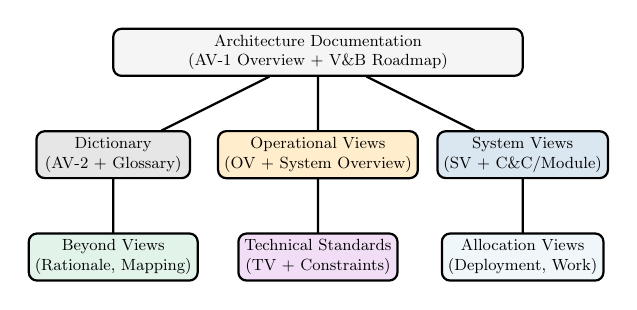
\begin{tikzpicture}[
    scale=0.65,
    transform shape,
    doc/.style={draw, thick, fill=#1, minimum width=3cm, minimum height=0.9cm, rounded corners=3pt, font=\small, align=center},
    arrow/.style={-{Stealth[length=2mm]}, thick}
]
    % Top level
    \node[doc=lightgray, minimum width=8cm] (title) at (0,5) {Architecture Documentation\\(AV-1 Overview + V\&B Roadmap)};
    
    % Second level
    \node[doc=allviewcolor!20] (dict) at (-4,3) {Dictionary\\(AV-2 + Glossary)};
    \node[doc=opviewcolor!20] (ops) at (0,3) {Operational Views\\(OV + System Overview)};
    \node[doc=svviewcolor!20] (sys) at (4,3) {System Views\\(SV + C\&C/Module)};
    
    % Third level
    \node[doc=vbcolor!15] (beyond) at (-4,1) {Beyond Views\\(Rationale, Mapping)};
    \node[doc=tvviewcolor!20] (tech) at (0,1) {Technical Standards\\(TV + Constraints)};
    \node[doc=alloccolor!20] (alloc) at (4,1) {Allocation Views\\(Deployment, Work)};
    
    % Connections
    \draw[thick] (title) -- (dict);
    \draw[thick] (title) -- (ops);
    \draw[thick] (title) -- (sys);
    \draw[thick] (dict) -- (beyond);
    \draw[thick] (ops) -- (tech);
    \draw[thick] (sys) -- (alloc);
\end{tikzpicture}
\caption{Integrated Documentation Structure}
\end{figure}

%==============================================================================
\section{Complete Mapping Reference}
%==============================================================================

\begin{longtable}{@{}L{1.2cm} L{1cm} L{3cm} L{3.5cm} L{3.8cm}@{}}
\caption{Complete DoDAF to Views and Beyond Mapping} \\
\toprule
\textbf{Category} & \textbf{ID} & \textbf{DoDAF Product} & \textbf{Description} & \textbf{V\&B Equivalent} \\
\midrule
\endfirsthead
\toprule
\textbf{Category} & \textbf{ID} & \textbf{DoDAF Product} & \textbf{Description} & \textbf{V\&B Equivalent} \\
\midrule
\endhead
\bottomrule
\endlastfoot

% All View
\multirow{2}{*}{All View} 
& AV-1 & Overview and Summary & Scope, purpose, findings & Documentation roadmap; System overview; Rationale \\
& AV-2 & Integrated Dictionary & Term definitions & Glossary \\
\midrule

% Operational
\multirow{8}{*}{Operational}
& OV-1 & Operational Concept & High-level concept graphic & System overview \\
& OV-2 & Resource Flow & Node connectivity & Context diagram \\
& OV-3 & Resource Flow Matrix & Information exchange & C\&C view \\
& OV-4 & Organizational Chart & Organization relations & Work assignment view \\
& OV-5 & Activity Model & Activities and flows & Behavior documentation \\
& OV-6a & Rules Model & Business rules & Behavior documentation \\
& OV-6b & State Transition & Event responses & Behavior documentation \\
& OV-6c & Event-Trace & Scenarios & Behavior documentation \\
& OV-7 & Logical Data Model & Data requirements & Data model view; Behavior \\
\midrule

% Systems and Services
\multirow{12}{*}{\makecell[l]{Systems \&\\Services}}
& SV-1 & Interface Description & Systems/services interconnections & C\&C views \\
& SV-2 & Communications & Communications laydown & C\&C views; Deployment \\
& SV-3 & Matrix & Relations among systems & Mapping between views \\
& SV-4a & System Functionality & System functions & Decomposition view \\
& SV-4b & Service Functionality & Service functions & Decomposition view \\
& SV-5a & Activity-Function Trace & Function traceability & Requirements mapping \\
& SV-5b & Activity-System Trace & System traceability & Requirements mapping \\
& SV-5c & Activity-Service Trace & Service traceability & Requirements mapping \\
& SV-6 & Data Exchange Matrix & Data exchange details & C\&C views; Interface docs \\
& SV-7 & Measures Matrix & Performance characteristics & Element catalog; QA docs \\
& SV-8 & Evolution & Migration plans & Rationale; Variability \\
& SV-9 & Technology Forecast & Emerging technologies & Rationale \\
& SV-10a & Rules Model & System constraints & Behavior in C\&C \\
& SV-10b & State Transition & System state responses & Behavior in C\&C \\
& SV-10c & Event-Trace & System sequences & Behavior in C\&C \\
& SV-11 & Physical Schema & Physical data model & Data model view \\
\midrule

% Technical Standards
\multirow{2}{*}{\makecell[l]{Technical\\Standards}}
& TV-1 & Standards Profile & Applicable standards & Element catalog relations \\
& TV-2 & Standards Forecast & Emerging standards & Element catalog; Rationale \\

\end{longtable}

%==============================================================================
\section{Appendix A: Checklist for DoDAF Compliance}
%==============================================================================

\begin{checklistbox}[DoDAF Compliance Checklist Using Views and Beyond]

\textbf{All Viewpoint:}
\begin{itemize}[leftmargin=1.5cm]
    \item[$\square$] AV-1: Documentation roadmap created
    \item[$\square$] AV-1: System overview documented
    \item[$\square$] AV-1: Analytical findings in rationale
    \item[$\square$] AV-2: Glossary complete
    \item[$\square$] AV-2: All terms defined
\end{itemize}

\textbf{Operational Viewpoint:}
\begin{itemize}[leftmargin=1.5cm]
    \item[$\square$] OV-1: System overview includes operational concept
    \item[$\square$] OV-2: Context diagrams for operational nodes
    \item[$\square$] OV-3: C\&C view shows information exchange
    \item[$\square$] OV-4: Work assignment view includes organizations
    \item[$\square$] OV-5/6/7: Behavior documented as needed
\end{itemize}

\textbf{Systems and Services Viewpoint:}
\begin{itemize}[leftmargin=1.5cm]
    \item[$\square$] SV-1: C\&C views show systems and services
    \item[$\square$] SV-2: Communications in C\&C and deployment views
    \item[$\square$] SV-3: View mappings documented
    \item[$\square$] SV-4: Decomposition views for functionality
    \item[$\square$] SV-5: Requirements mapping complete
    \item[$\square$] SV-6/7: Performance in element catalogs
    \item[$\square$] SV-8/9: Evolution in rationale
    \item[$\square$] SV-10: Behavior in C\&C views
    \item[$\square$] SV-11: Physical data model view
\end{itemize}

\textbf{Technical Standards Viewpoint:}
\begin{itemize}[leftmargin=1.5cm]
    \item[$\square$] TV-1: Standards in element catalog relations
    \item[$\square$] TV-2: Emerging standards noted
\end{itemize}
\end{checklistbox}

%==============================================================================
\section{Appendix B: Glossary}
%==============================================================================

\begin{description}[leftmargin=3cm, style=nextline]
    \item[DoDAF] Department of Defense Architecture Framework; standardized approach for defense enterprise architectures
    \item[Views and Beyond] SEI approach to software architecture documentation
    \item[Viewpoint] DoDAF: category of related products; V\&B: conventions for view construction
    \item[Product] DoDAF term for a specific architecture model or artifact
    \item[View] Work product expressing architecture from a perspective
    \item[C\&C View] Component-and-Connector view showing runtime structure
    \item[Module View] View showing code-time structure
    \item[Allocation View] View showing mapping to environments
    \item[Element Catalog] Detailed specification of architectural elements
    \item[Operational Node] DoDAF: logical node performing activities
    \item[System Node] DoDAF: physical location hosting systems
\end{description}

%==============================================================================
\section{Appendix C: References}
%==============================================================================

\begin{enumerate}
    \item Department of Defense. (2009). \textit{DoDAF Architecture Framework Version 2.02}.
    
    \item Clements, P., et al. (2010). \textit{Documenting Software Architectures: Views and Beyond} (2nd ed.). Addison-Wesley.
    
    \item Department of Defense. (2010). \textit{DoD Architecture Framework Version 2.0: Architect's Guide}.
    
    \item ISO/IEC/IEEE 42010:2011. \textit{Systems and software engineering---Architecture description}.
    
    \item Bass, L., Clements, P., \& Kazman, R. (2021). \textit{Software Architecture in Practice} (4th ed.). Addison-Wesley.
    
    \item The Open Group. (2018). \textit{TOGAF Standard, Version 9.2}. Van Haren Publishing.
    
    \item Rozanski, N., \& Woods, E. (2011). \textit{Software Systems Architecture} (2nd ed.). Addison-Wesley.
    
    \item INCOSE. (2015). \textit{Systems Engineering Handbook} (4th ed.). Wiley.
\end{enumerate}

\end{document}